%第3-4章
\section{詳細設計}
詳細設計では、3.3節の基本設計を受けて、より詳細なシステムの設計を行った。ここでは、時系列に沿ったオブジェクト間のメッセージのやり取りを確認するためにシーケンス図を作成し、アクティビティ図の作成の際と同じように、「室内環境を監視する(図\ref{s_kansi})」、「換気要請の受け取り(図\ref{s_kanki})」、「入室危険度の確認(図\ref{s_nyuusitu})」、「室内環境状態の表示(図\ref{s_situnaikankyou})」の4つのユースケースについて、より詳細な処理の流れを確認した。以下に作成したシーケンス図を示す。


\begin{figure}[H]
	\centering
	\includegraphics[width=15cm]{s_kansi.eps}
	\caption{室内環境を監視する}
	\label{s_kansi}
\end{figure}
\begin{figure}[H]
	\centering
	\includegraphics[width=15cm]{s_kanki.eps}
	\caption{換気要請の受け取り}
	\label{s_kanki}
\end{figure}
\begin{figure}[H]
	\centering
	\includegraphics[width=15cm]{s_nyuusitu.eps}
	\caption{入室危険度の確認}
	\label{s_nyuusitu}
\end{figure}
\begin{figure}[H]
	\centering
	\includegraphics[width=15cm]{s_situnaikankyou.eps}
	\caption{室内環境状態の表示}
	\label{s_situnaikankyou}
\end{figure}

ここでは、各ユースケースのより具体的な処理の流れを確認することができた。ここまで少し曖昧さがあった点についても、突き詰めて考えることができている。

例えば、ここまでの段階で、どのような情報をどのように収集するかというところまでは議論が進められていた。しかし、信頼性の高い結果を導き出すために、また、論理的に情報を分析するためには情報収集と分析にもルールを定める必要がある。例えば、複数のセンサデバイスの値を平均した値が部屋の換気状態を表しているといえるかという点に関しては、二酸化炭素は気体の一種であることから、部屋中に一様に広がっているとは言えず、風の流れなどにも場所によって差が出ると考えられることから、部屋の中で特に換気状態が悪い箇所の値を、その部屋の換気状態を表す値として見ることが、感染症予防の観点から考えても、妥当だと考えた。

また、室内に滞在する人の数が極端に少なくなれば、多くの人が室内に滞在していた時と比べ、二酸化炭素濃度が徐々に低下すると考えられるが、この場合にも、室内に大勢の人が滞在している場合と同じモニタリングをするようでは、その部屋の感染リスクの高まりやすさの傾向を掴むには不適切となると考えた。既に述べているがこのシステムでは、モニタリング開始前に、部屋の広さと、何平方メートルに1人が滞在できるかという部屋の運用ルールに従って、部屋に滞在できる最大人数を定めている。この人数の75\%以上の人数が、室内に滞在していない状態になれば警戒レベルや感染リスクの導出は行わず、二酸化炭素濃度値を安全水準(ここでは700ppmとしている)まで下げるよう換気要請のみを行うこととした。

シーケンス図の作成によって、それぞれのユースケースでの処理の流れがより詳細となった。先ほど述べた内容以外にも、センサデバイス側の消費電力を抑える関係で、モニタリング開始時にJetson nano側から開始命令が出された後には、センサデバイスは基本的に受信状態には入らず、3分経過ごとにデータの取得・送信を繰り返し行うことや、一定期間のデータの参照の必要性からデータベースを用いることなどが、より詳細な設計として確認された。アクティビティ図でもこのような流れを大まかに掴むことはできていたが、より詳細に設計が進み、実装の際の課題となり得る点もいくつか発見された。

また、以上の詳細設計の内容をもとに、単体テスト項目として表\ref{jtantaitest_koumoku}、\ref{dtantaitest_koumoku}の項目を挙げた。

\begin{table}[H]
	\centering
	\caption{エッジサーバ(Jetson nano)側 単体テスト項目}
	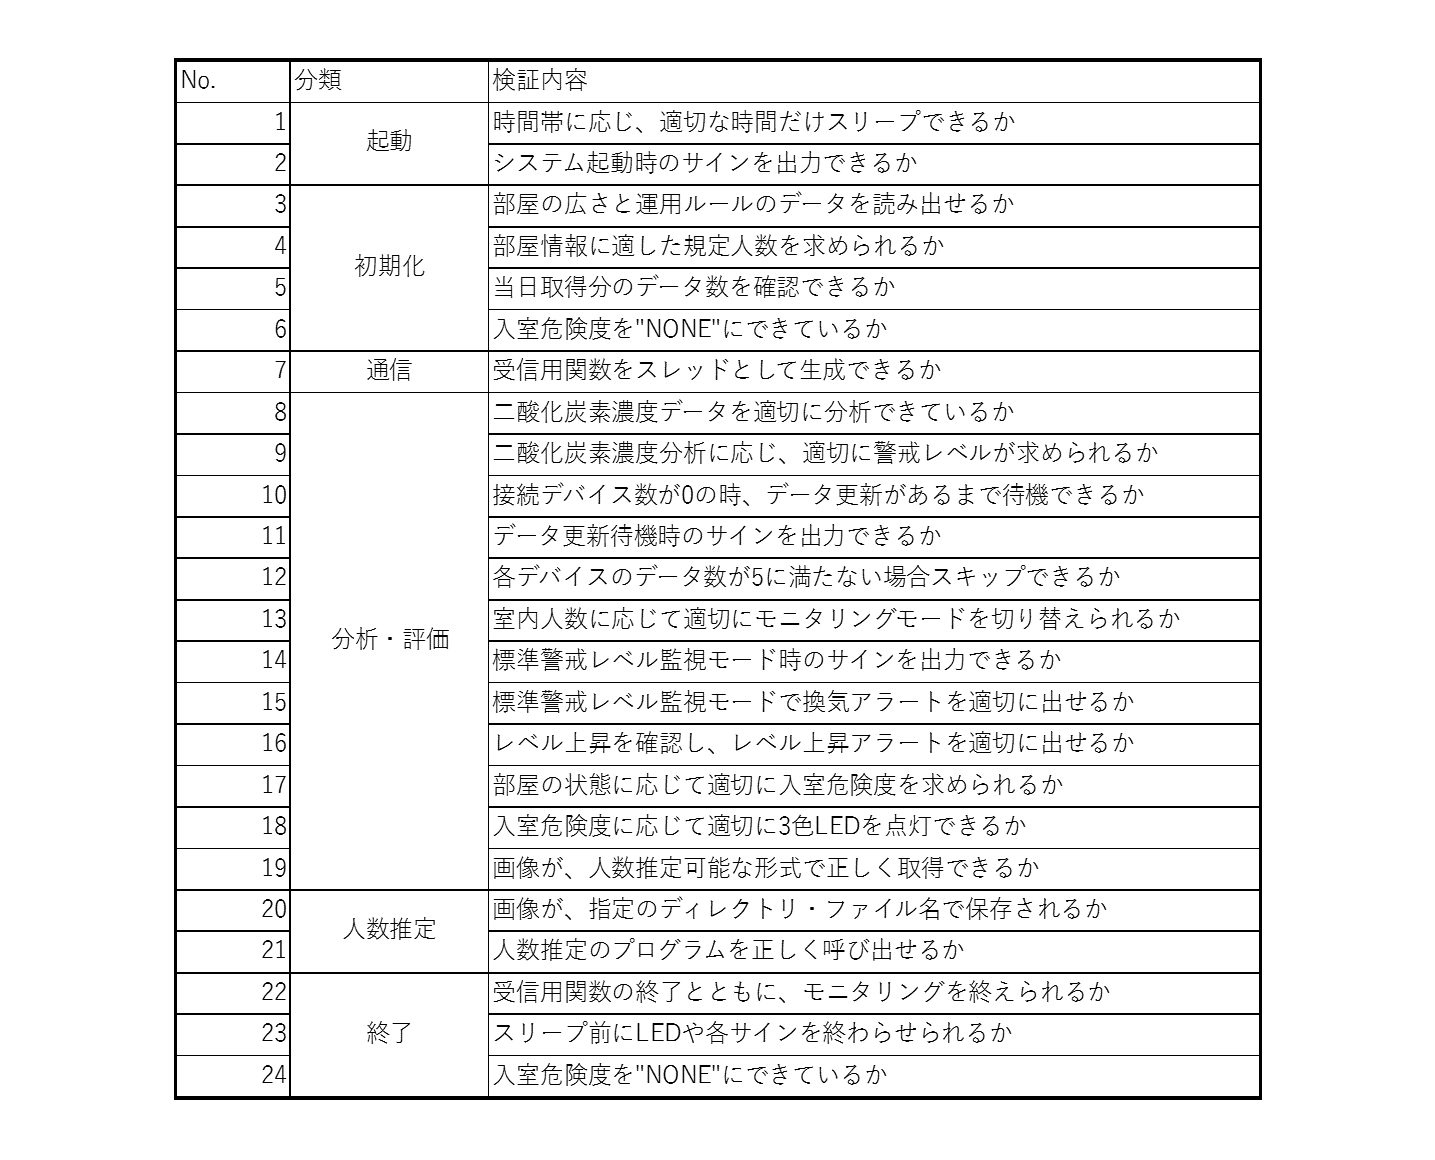
\includegraphics[width=15cm]{jtantaitest_koumoku.eps}
	\label{jtantaitest_koumoku}
\end{table}

\begin{table}[H]
	\centering
	\caption{データベース 単体テスト項目}
	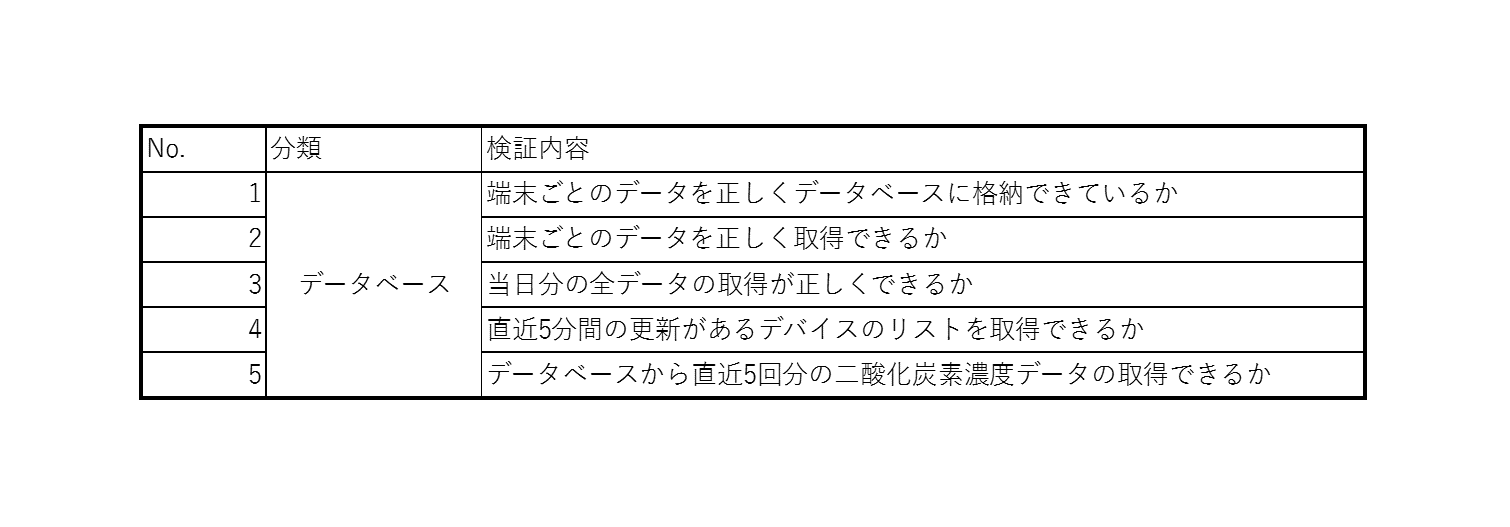
\includegraphics[width=15cm]{dtantaitest_koumoku.eps}
	\label{dtantaitest_koumoku}
\end{table}

詳細設計を終え、私たちはこれまでの設計内容や、発見された課題を踏まえ、いかにして対処するかを議論しつつ、実装を進めた。